\chapter{Evaluation of amplifiers} \label{chromosomes-evaluation}
A fitness function provides the means to determine how good the evolved solution is so that the most appropriate candidates can be distinguished from the less appropriate ones. It is important to mention that the quality of this function is essential because the ability of the algorithm to find the most suitable solution is highly dependent on the ability of the fitness function to distinguish between the individuals. The value of the function is a positive real number in our case and the algorithm uses it only for comparing the individuals between each other. We consider those individuals with the lower value as the better ones.

The implementation required some methods of trial and error and in the end, there are three fitness functions implemented in this thesis. All of them use the ngSPICE simulator in order to obtain the output of the amplifier and assess it afterwards. The simulation is done for every candidate solution and it takes most of the computation time of the overall evolutionary algorithm.

\section{Best match with the reference solution}
This fitness function has been implemented as the first one in order to find out if the evolution has at least the ability to get close to the analytical solution. It is based on the method of least squares which is used in regression analysis.

The fitness function uses the output voltage vector from the simulator for assessing the chromosomes. The vector represents the waveform of the output signal from the circuit and the shape of the waveform gets similar to an inverted sine wave as the solution evolves. The length of the vector is set to 69 (the sampling period is approximately \SI{20}{\micro\second}) elements during the whole evolution and the vector contains approximately 2.5 periods of the signal (the signal's frequency is \SI{20}{\kilo\hertz}). The fitness function uses two types of these vectors, one serves as the reference vector (the output of the amplifier which elements' values were calculated analytically) and all the candidate vectors are compared to it. As we can see in figure \ref{ce-amplifier-sim}, the first period of the signal is unstable, so the fitness function skips it and picks only the second period for comparison with the reference signal. It is sufficient to compare only the second period because the shape of the signal doesn't change anymore after the circuit gets to a stable state.

The functions in algorithm \ref{get-second-period} are used to extract the second period from the waveform. Since the vector has a constant length and the values represent an inverted sine wave, we can walk through the first two and the last half-period to get to the desired part of the signal.

The first function starts at the start of the vector and it skips the first half-period which values are less than zero and it also skips the second half-period in a similar way. The second function starts from the end of the vector and it skips the second last period of the signal in the vector. The resulting $start$ and $end$ indices point to the start and the end of the second period of the signal.

When the evolution starts, the waveform of some candidate solutions is not in the shape of an inverted sine wave and therefore it crosses zero sooner than the desired waveform. In this case, the algorithm ends with indices close to the starting and ending index and such candidate solution is assessed with a high fitness value.

    \begin{algorithm}
    \caption{Find the first and last index of the second period}
    \label{get-second-period}
    \begin{algorithmic}[1]
        \Function{getStart}{$vector$}
            \State $start \gets 0$;
            \While{$vector[start] < 0$}
                \State $start \gets start + 1$;
            \EndWhile
            \While{$vector[start] > 0$}
                \State $start \gets start + 1$;
            \EndWhile
            \State \Return $start$;
        \EndFunction
        \State

        \Function{getEnd}{$vector$}
            \State $end \gets vector.length()$;
            \While{$vector[end] < 0$}
                \State $end \gets end - 1$;
            \EndWhile
            \State \Return $end$;
        \EndFunction
    \end{algorithmic}
    \end{algorithm}

The function in algorithm \ref{bestFit} is used to evaluate the candidate solutions. It iterates over the second period in both reference and candidate vectors and it calculates the sum of squares which sides are defined by the difference between the values in the reference vector and the candidate vector. The overall sum is returned as the result of the fitness function and the lower the value, the better the candidate solution is.

The reason why we add up squares and not only the absolute values of the differences is important. Consider two imaginary vectors of two values which differ from the reference vector by $(1, 5)$ and by $(3,3)$. The sum of the absolute values is 6 in both cases, so this method doesn't distinguish between these vectors. However, the sum of the squares is 26 for the first vector and 18 for the second one. This difference is important as we want all the values to be close to the reference and not only some of them and therefore the second vector is assessed as the better one.

\begin{algorithm}
\caption{Fitness evaluation using the analytical solution}
\label{bestFit}
\begin{algorithmic}[1]
    \Function{rateChromosome}{$candidateVector$, $referenceVector$}
        \State $fitness \gets 0$;
        \State $start \gets$ \Call{getStart}{$candidateVector$};
        \State $end \gets$ \Call{getEnd}{$candidateVector$};
        \For{$i \gets start : end$}
            \State $fitness \gets fitness + (referenceVector[i] - candidateVector[i])^2$;
        \EndFor
        \State \Return $fitness$;
     \EndFunction
\end{algorithmic}
\end{algorithm}

We can see the result of the evolution using this fitness function in figure \ref{best-match}.

\begin{figure}[H]
    \centerline{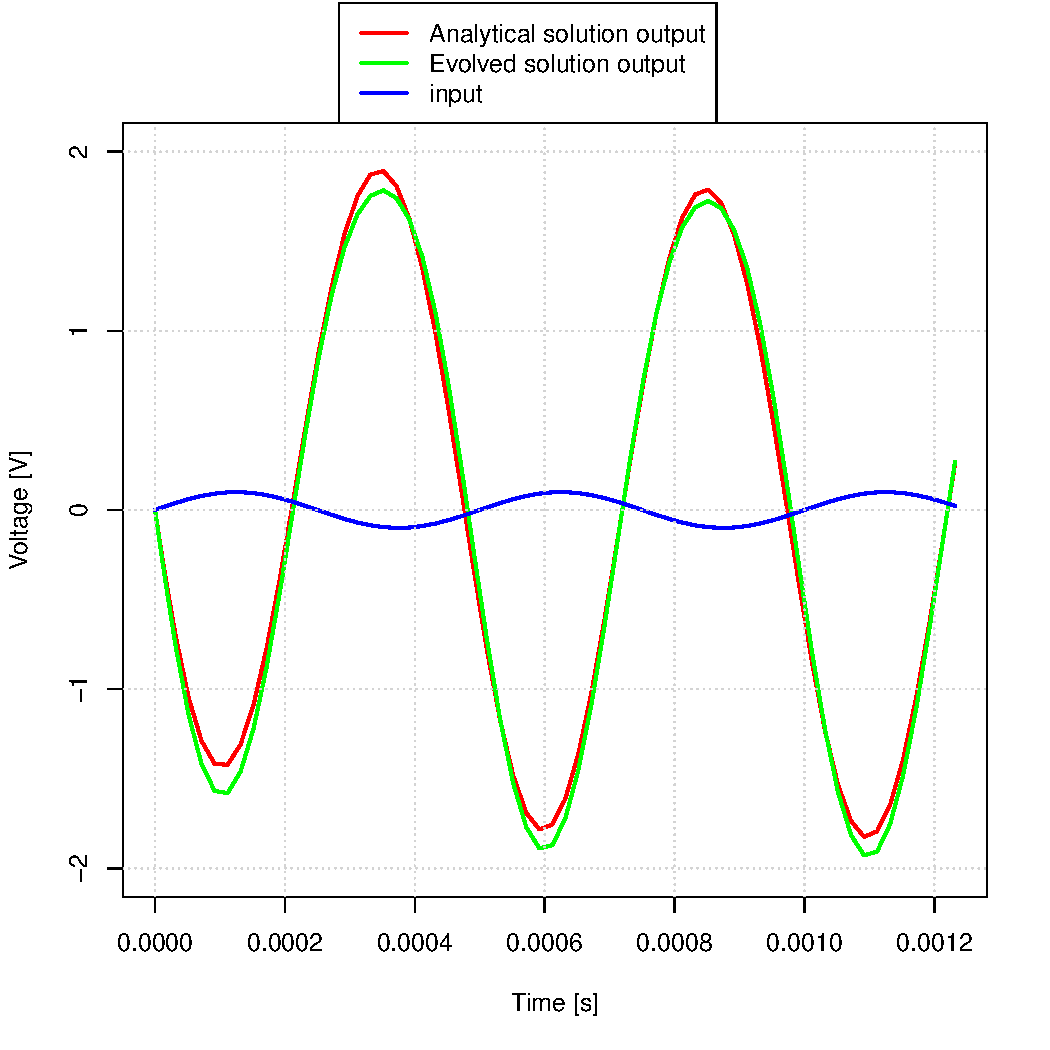
\includegraphics[scale=0.6]{best-match}\label{best-match}}
    \caption{The result of evolution towards the analytical solution}
\end{figure}

\section{Ideal sine wave}
This method is similar to the previous one but instead of using the pre-simulated output as a reference, it uses an analytically calculated sine wave. An analytical sine wave is used in order to force the evolution towards such solution that won't produce a distorted output signal since the input is in the form of a sine wave as well. The function also uses the method of least squares explained in the previous section and it iterates over the second period of the signal which is represented by the $candidateVector$.

We can see the technique in algorithm \ref{idealSine}. In every iteration, it calculates the value of the sine wave and compares it with the simulated signal. The sum of the comparisons is then returned as the fitness value and the lower the result is, the closer the candidate solution is to the reference. The amplitude of the sine wave is set by the user, so this method allows users to design amplifiers with an arbitrary amplification which doesn't exceed the circuit's capabilities.

\begin{algorithm}[H]
\caption{Fitness evaluation using the ideal sine wave}
\label{idealSine}
\begin{algorithmic}[1]
    \Function{rateChromosome}{$candidateVector$, $amplitude$}
        \State $fitness \gets 0$;
        \State $start \gets$ \Call{getStart}{$candidateVector$};
        \State $end \gets$ \Call{getEnd}{$candidateVector$};
        \State $refSineSize \gets end - start$;
        \For{$i \gets 0 : refSineSize$}
           \State \scalebox{1.3}{$refSine \gets -amplitude \cdot \sin(\frac{2 \pi i}{refSineSize - 1})$};
           \State $fitness \gets fitness + (refSine - candidateVector[start + i])^2$;
        \EndFor
        \State \Return $fitness$;
    \EndFunction
\end{algorithmic}
\end{algorithm}

\section{Maximal amplitude}
This fitness function is designed to rate the candidate solutions only according to the amplitude of the output regardless of the waveform's shape. It can be used for finding the highest amplification capabilities of the circuit. The function finds the trough and the peak in the second period and returns the multiplicative inverse of their difference.

\begin{algorithm}[H]
\caption{Rating the chromosomes according to the amplitude}
\label{maxAmp}
\begin{algorithmic}[1]
    \Function{rateChromosome}{$candidateVector$}
        \State $start \gets$ \Call{getStart}{$candidateVector$};
        \State $end \gets$ \Call{getEnd}{$candidateVector$};
        \State $trough \gets \min(candidateVector[start]$, $candidateVector[end])$;
        \State $peak \gets \max(candidateVector[start]$, $candidateVector[end])$;
        \State \Return \scalebox{1.2}{$\frac{1}{peak - trough}$};
    \EndFunction
\end{algorithmic}
\end{algorithm}

\section{Waveform symmetry}
All of the fitness functions discussed above have difficulties in finding symmetrical waveforms. An example is shown in figure \ref{asymmetrical-ideal-sine}.

\begin{figure}[!ht]
    \centerline{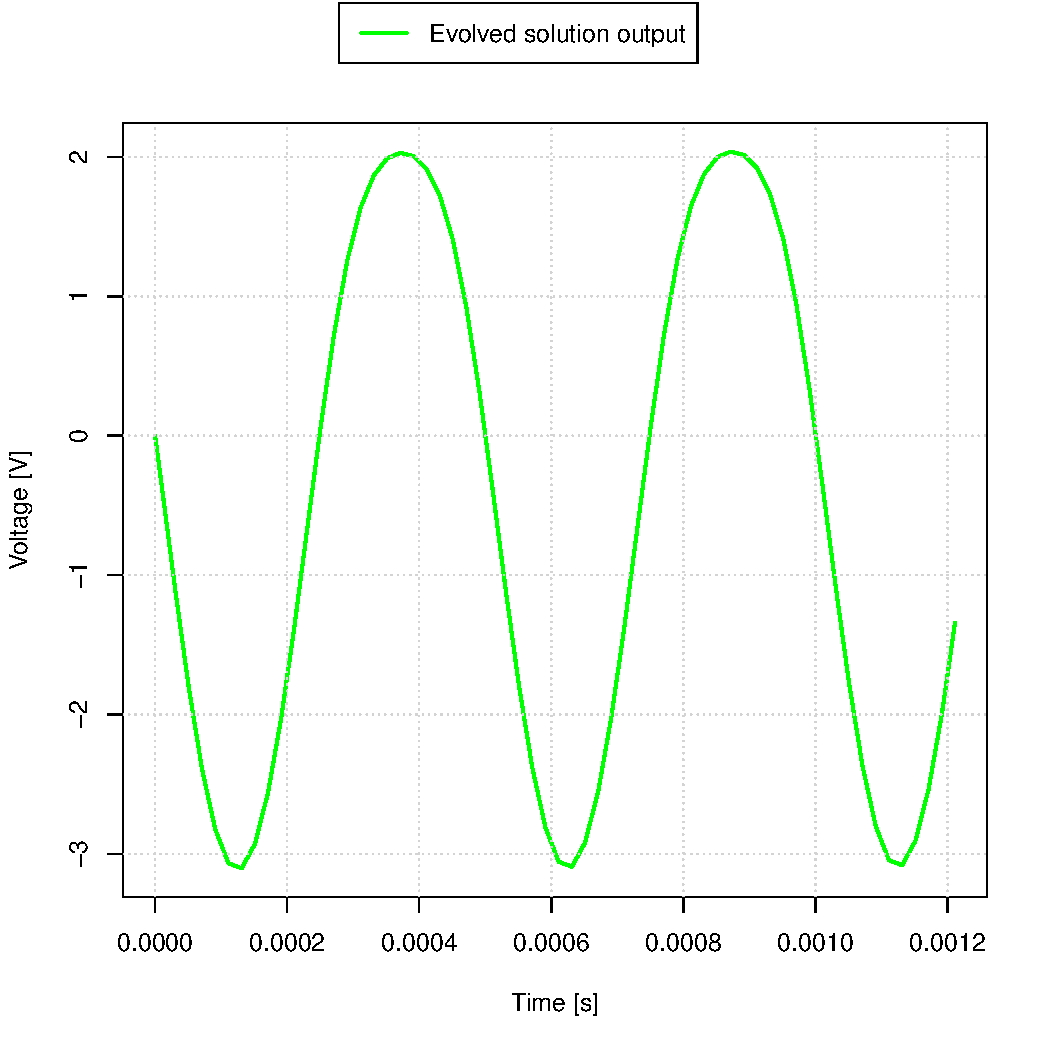
\includegraphics[scale=0.6]{asymmetrical-ideal-sine}\label{asymmetrical-ideal-sine}}
    \caption{An asymmetrical result of the evolution using the 'ideal sine wave' evaluation}
\end{figure}

The problem is that at the start, the output signal has zero power and as the evolution continues, only one half of the signal rises and the fitness function value decreases even though the evolution doesn't go in the right direction. At the end, the evolution ends up in the state shown in figure \ref{asymmetrical-ideal-sine}. The first solution to this problem is described in formula \ref{sym1}.

\begin{equation} \label{sym1}
result = (|peak + trough| + 1) \cdot fitness
\end{equation}

The $peak$ and $trough$ values are obtained in the same way as in algorithm \ref{maxAmp}. If the signal is symmetrical, the absolute value of the sum of these values is close to zero and therefore the $result$ will also be lower. We add 1 to the sum because we need to distinguish between perfectly symmetrical signals with different fitness. However, it emerged that this approach is too restrictive as it promotes only signals which are perfectly symmetrical, but often distorted. The result is shown in figure \ref{symmetrical-ideal-sine}.

\begin{figure}[!ht]
    \centerline{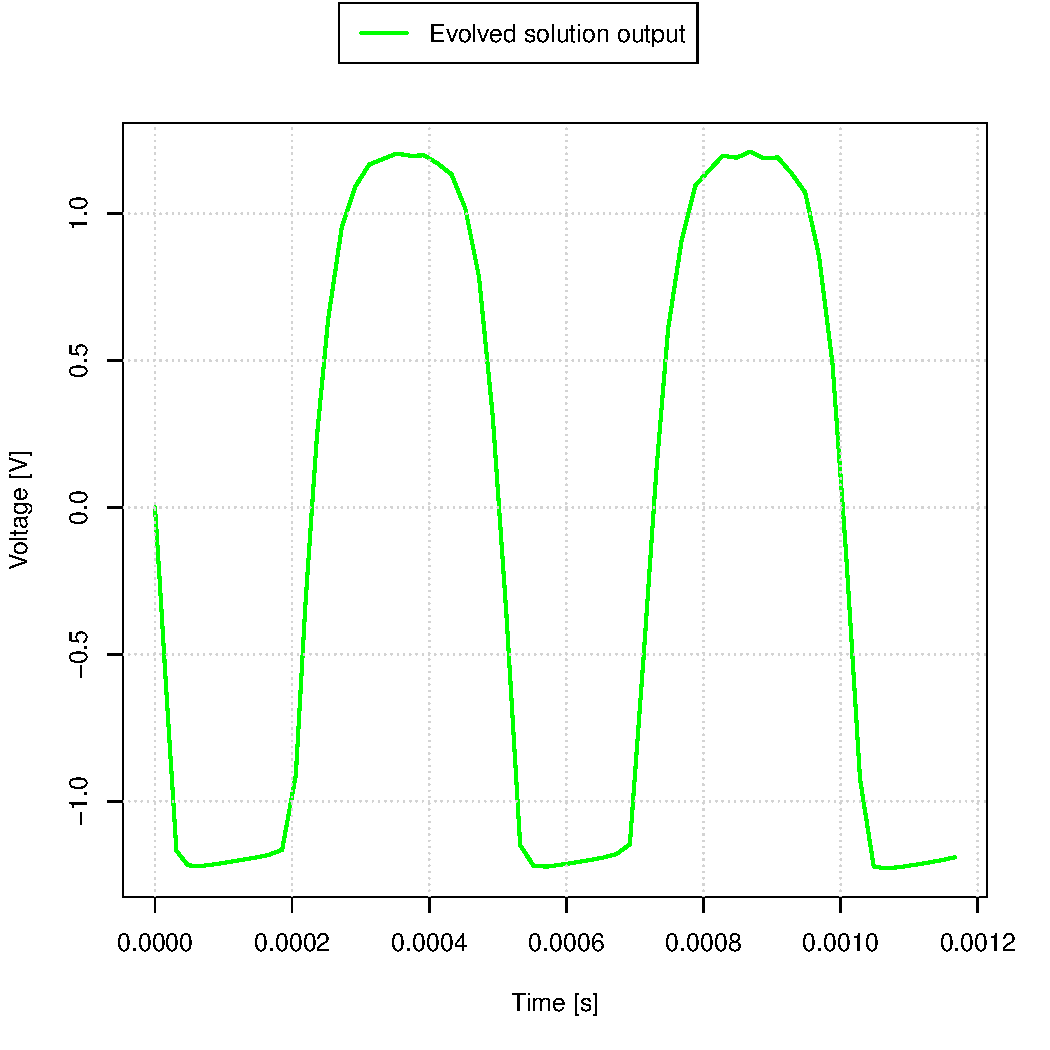
\includegraphics[scale=0.6]{symmetrical-ideal-sine}\label{symmetrical-ideal-sine}}
    \caption{A distorted result using the 'ideal sine wave' evaluation with perfect symmetry}
\end{figure}

The ability of the evolution to find the desired solution was also decreased because some asymmetrical candidate solutions head towards a good solution. These consequences led to another solution to this problem.

\begin{algorithm}
\caption{Rating the chromosomes with regard to the symmetry of the signal}
\label{symmetry-rating}
\begin{algorithmic}[1]
    \Function{rateChromosome}{$candidateVector$, $maxDifference$}
    \State $min \gets \min(|trough|$, $peak)$;
    \State $max \gets \max(|trough|$, $peak)$;
    \If{\scalebox{1.1}{$\frac{min}{max} < (1 - \frac{maxDifference}{100})$}}
        \State \Return $DOUBLE\_MAX$;
    \EndIf
    \LineComment{continue evaluating the chromosome}
    \EndFunction
\end{algorithmic}
\end{algorithm}

Condition on line 4 in algorithm \ref{symmetry-rating} is used to separate the symmetrical and asymmetrical chromosomes. The values of the variables $trough$ and $peak$ are obtained in the same way as in algorithm \ref{maxAmp}. The value of $maxDifference$ is in the interval $\left]0, 100\right]$ and it is set by the user. It represents the maximal percentage difference between the peak and trough in the second period of the signal. The algorithm calculates the ratio between the peak and trough and if the result is less than the threshold value, the chromosome is evaluated with the maximal fitness and the function is terminated. Otherwise, the evaluation continues. This allows the user to control the results of the evolution with respect to the symmetry of the output signal.